%%%%%%%%%%%%%%%%%%%%%%%%%%%%%%%%%%%%%%%%%%%%%%%%%%%%%%%%%%%%%%%%%%%%%%%%%%%%%%%%%%%%%%%%%%%%%%%%%%%%%%%%%%%%%%%%%%%%%%%%%%%%%%%%%%%%%%%%%%%%%%%%%%%%%%%%%%%
% BAMNet Supplementary Material
% Joint Aortic Root Segmentation and Landmark Localization on Intraoperative Fluoroscopy for TAVI Guidance
%%%%%%%%%%%%%%%%%%%%%%%%%%%%%%%%%%%%%%%%%%%%%%%%%%%%%%%%%%%%%%%%%%%%%%%%%%%%%%%%%%%%%%%%%%%%%%%%%%%%%%%%%%%%%%%%%%%%%%%%%%%%%%%%%%%%%%%%%%%%%%%%%%%%%%%%%%%

\documentclass[utf8]{frontiers_suppmat}
\usepackage{graphicx}
\usepackage{booktabs}
\usepackage{multirow}
\usepackage{amsmath,amssymb}
\usepackage{url,hyperref,lineno,microtype}
\usepackage[onehalfspacing]{setspace}

\begin{document}
\onecolumn
\firstpage{1}

\title[Supplementary Material]{{\helveticaitalic{Supplementary Material}}}

\maketitle

\section{Supplementary Figures}

\begin{figure}[htbp]
\centering
\begin{minipage}[b]{0.48\textwidth}
\centering
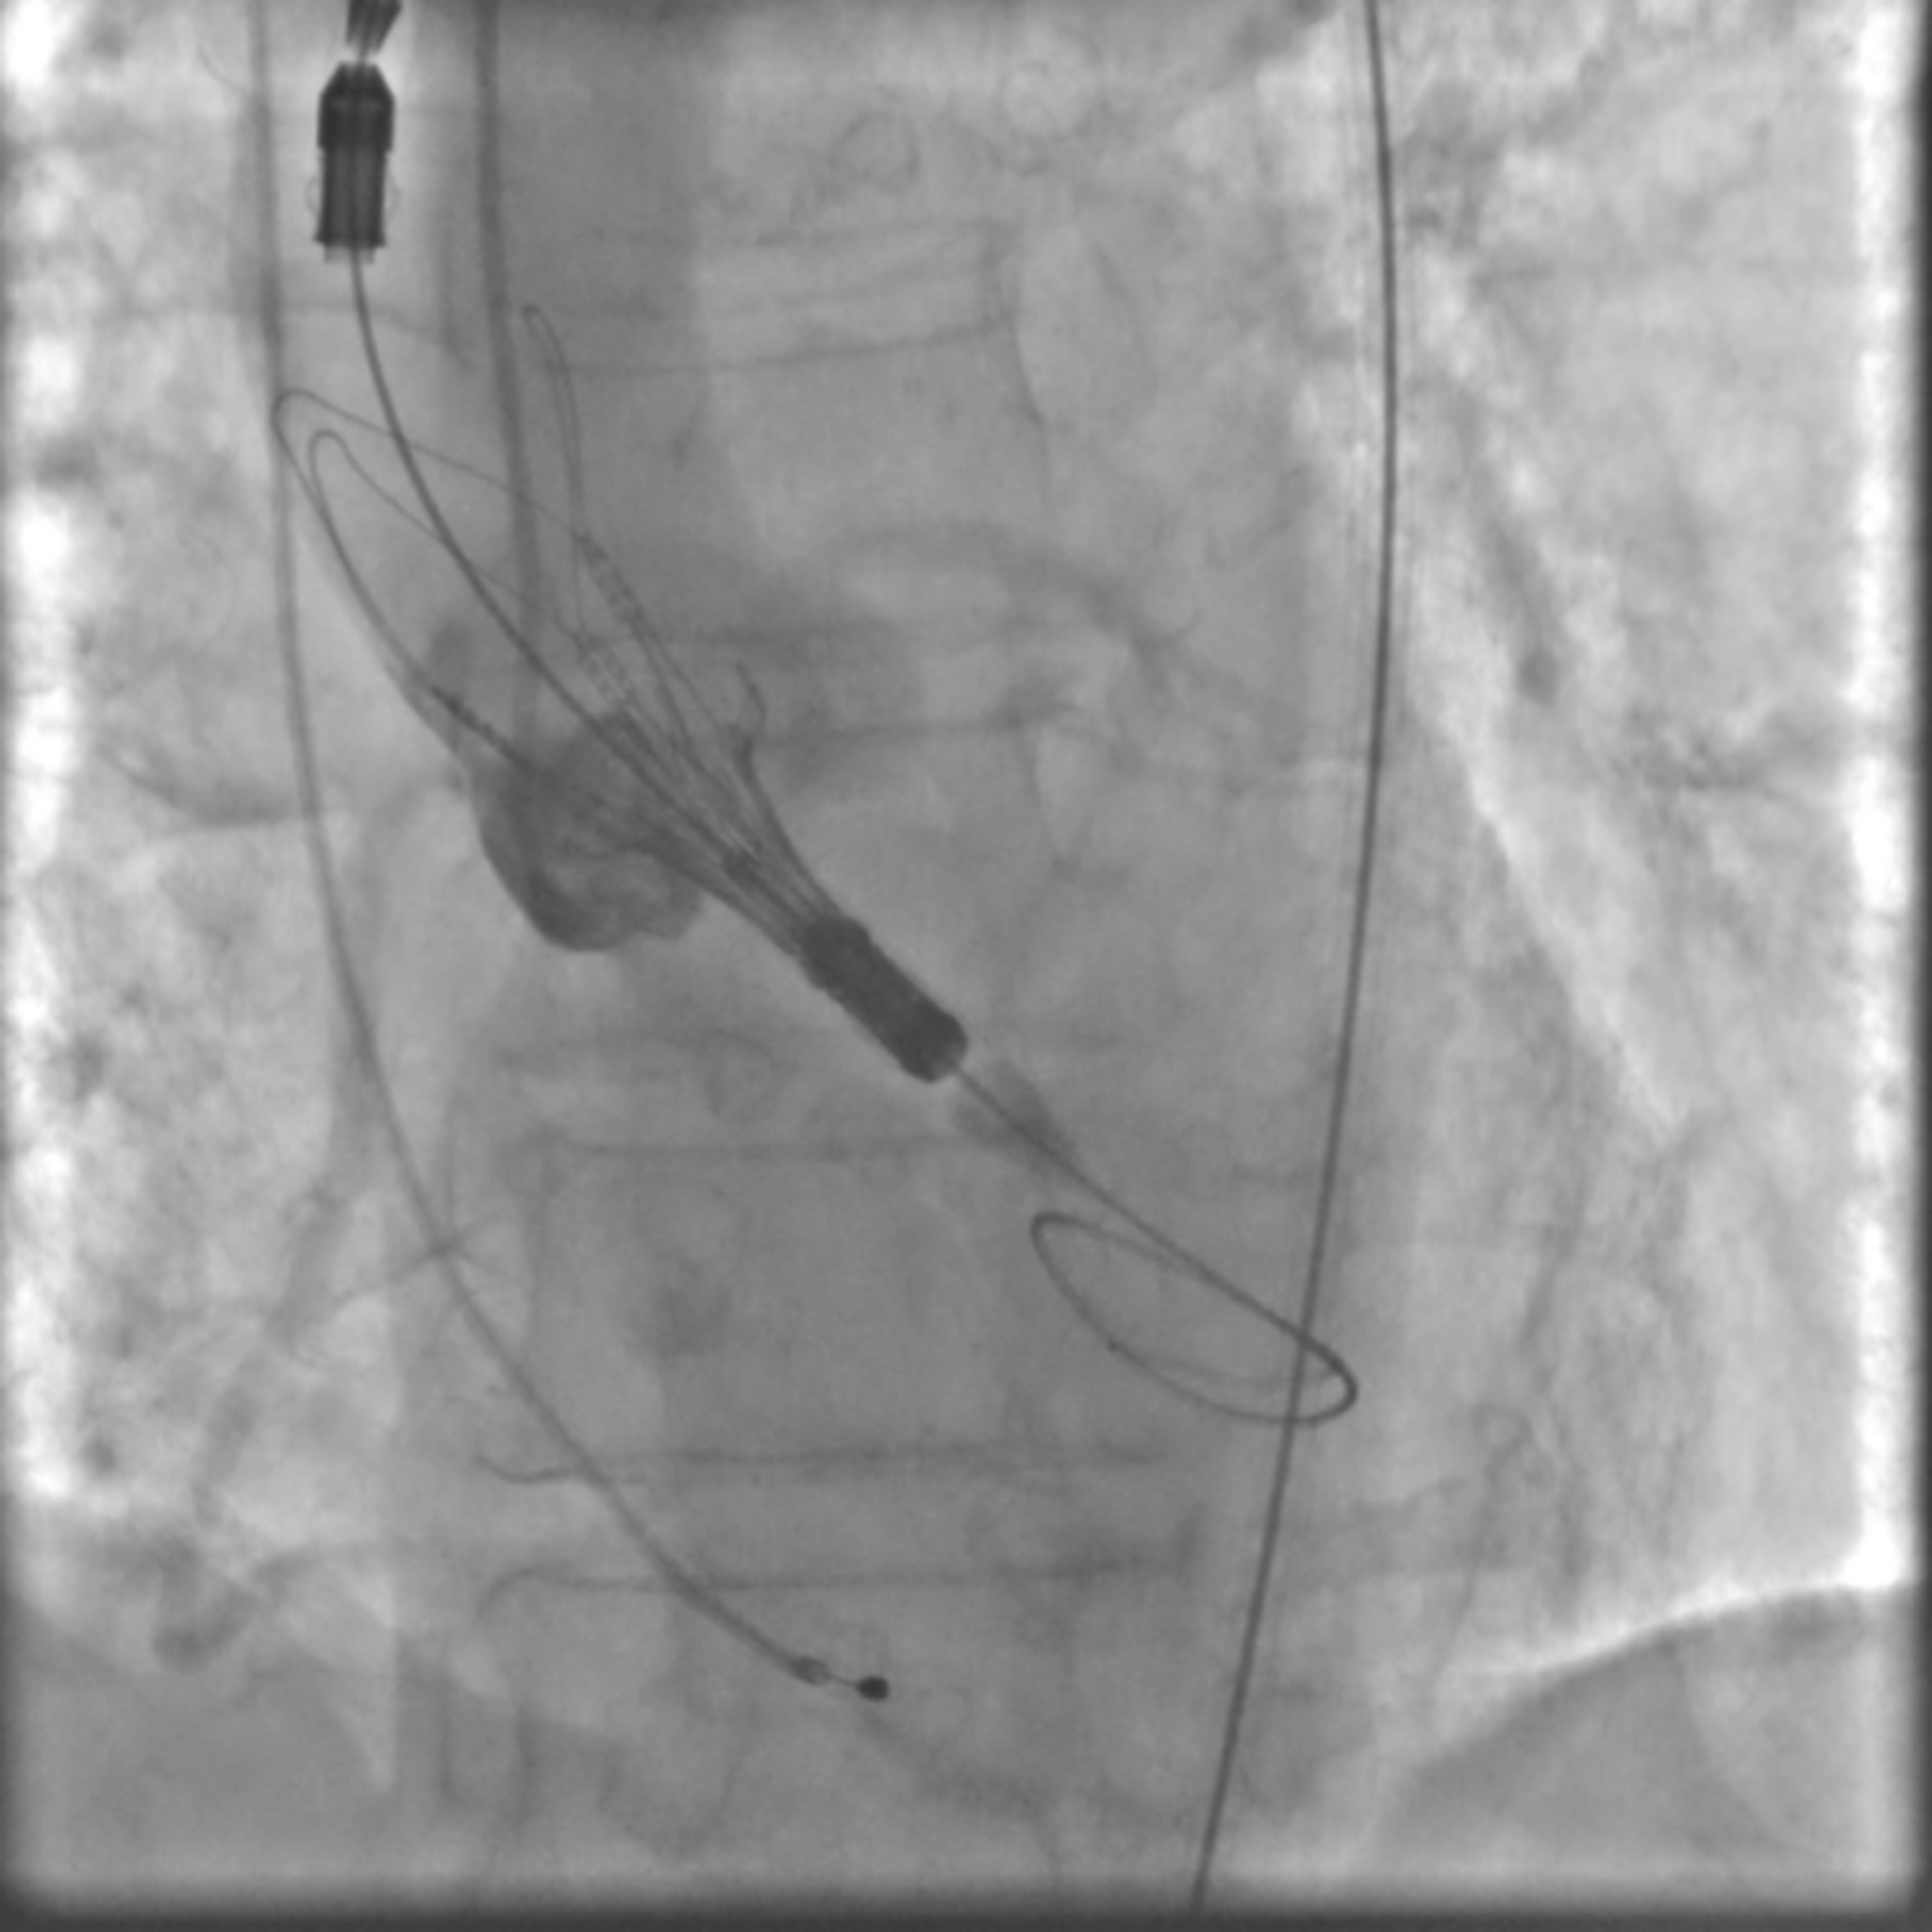
\includegraphics[width=\linewidth]{figures/Figure_1a.png}
\end{minipage}
\hfill
\begin{minipage}[b]{0.48\textwidth}
\centering
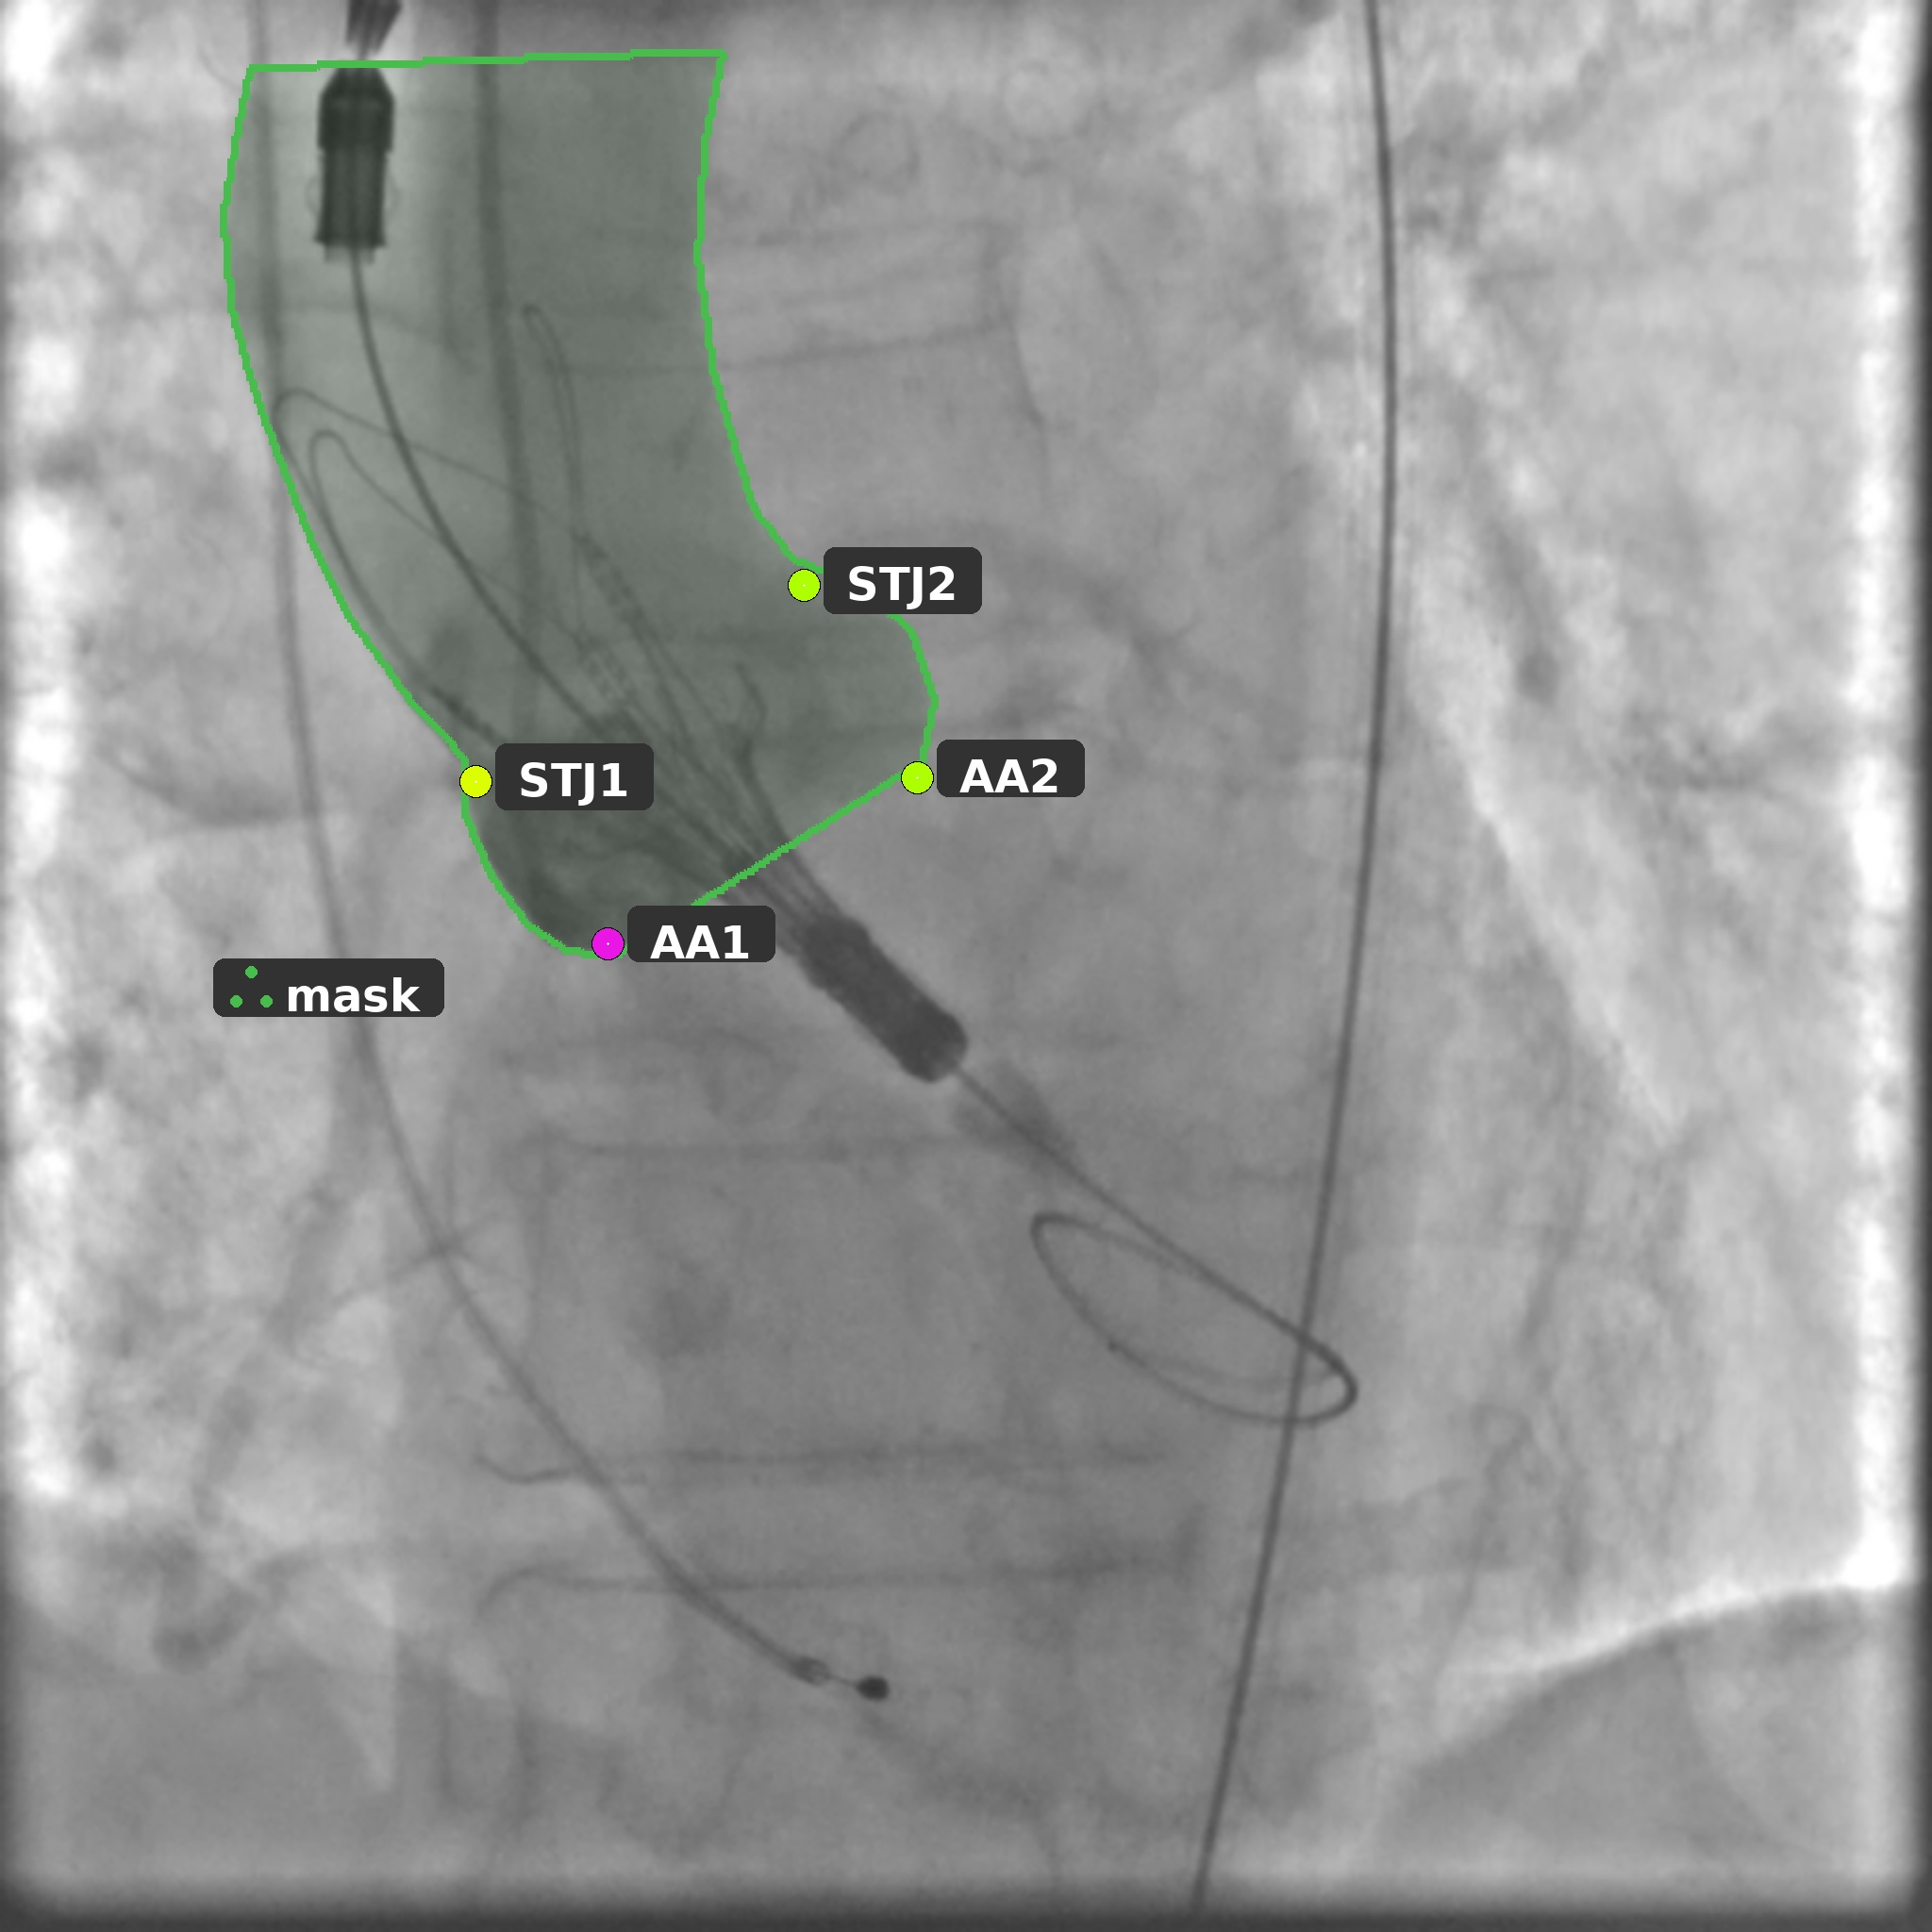
\includegraphics[width=\linewidth]{figures/Figure_1b.jpeg}
\end{minipage}

\begin{minipage}[b]{0.48\textwidth}
\centering
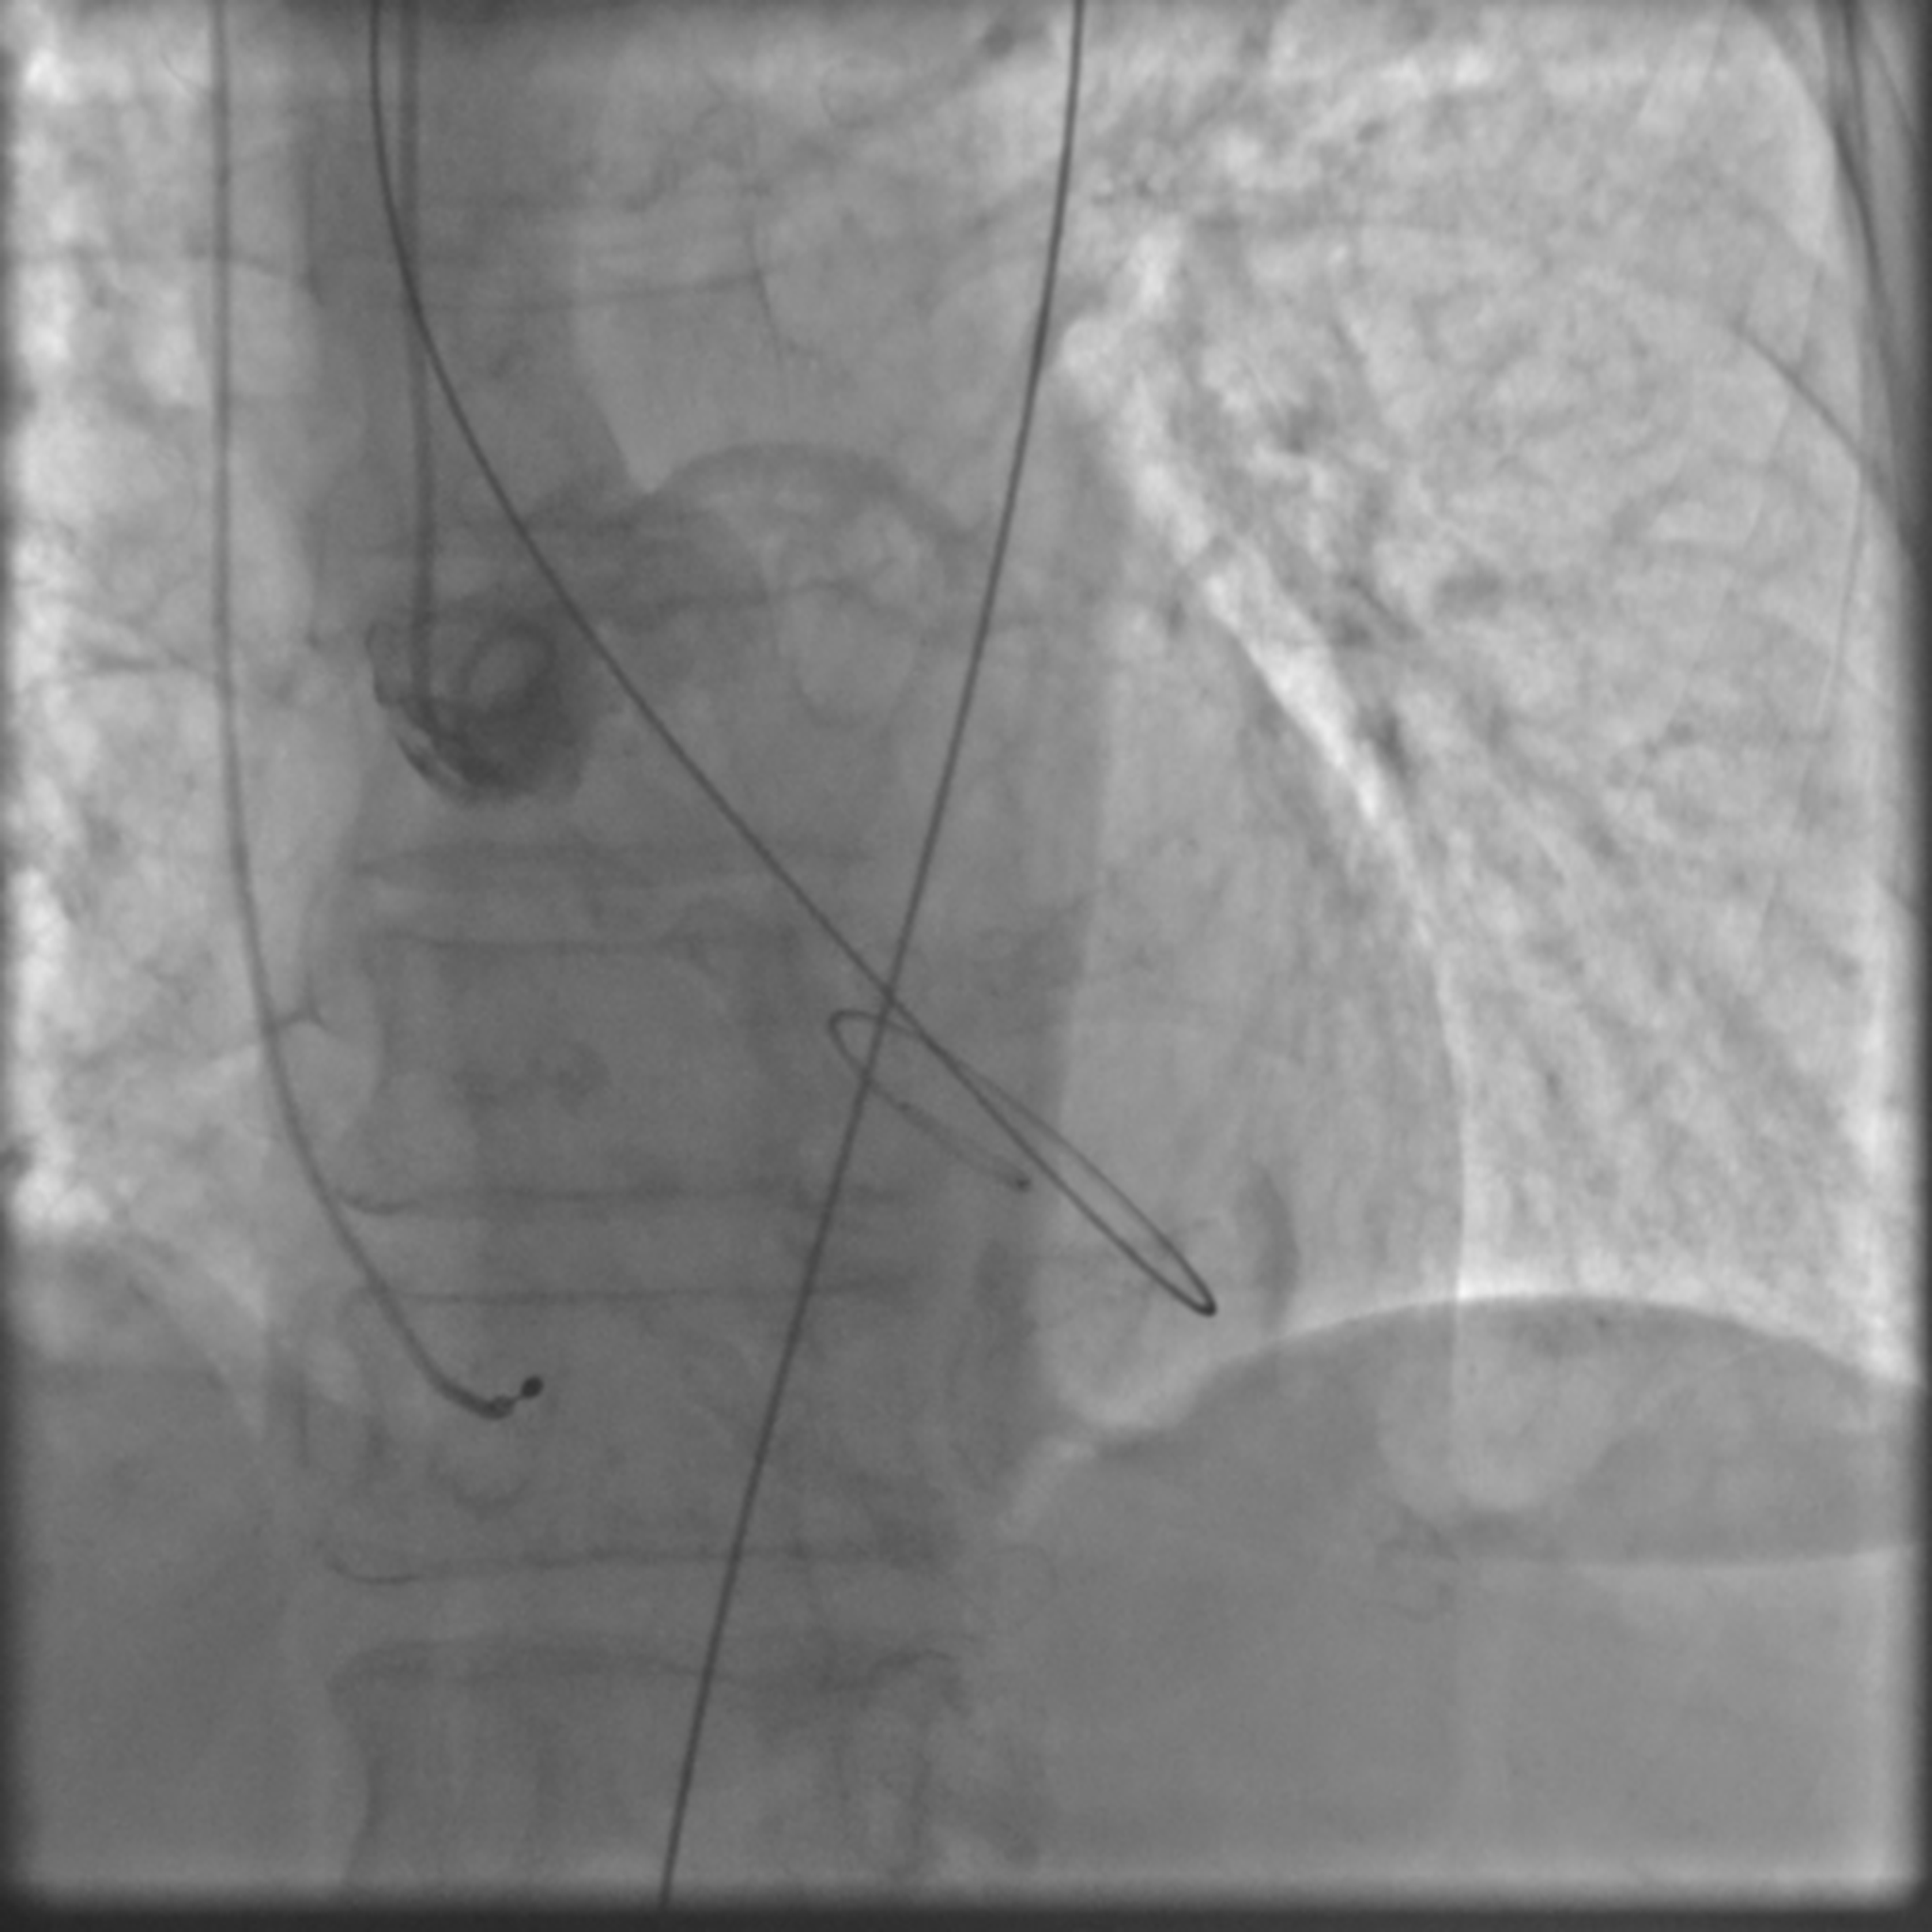
\includegraphics[width=\linewidth]{figures/Figure_1c.png}
\end{minipage}
\hfill
\begin{minipage}[b]{0.48\textwidth}
\centering
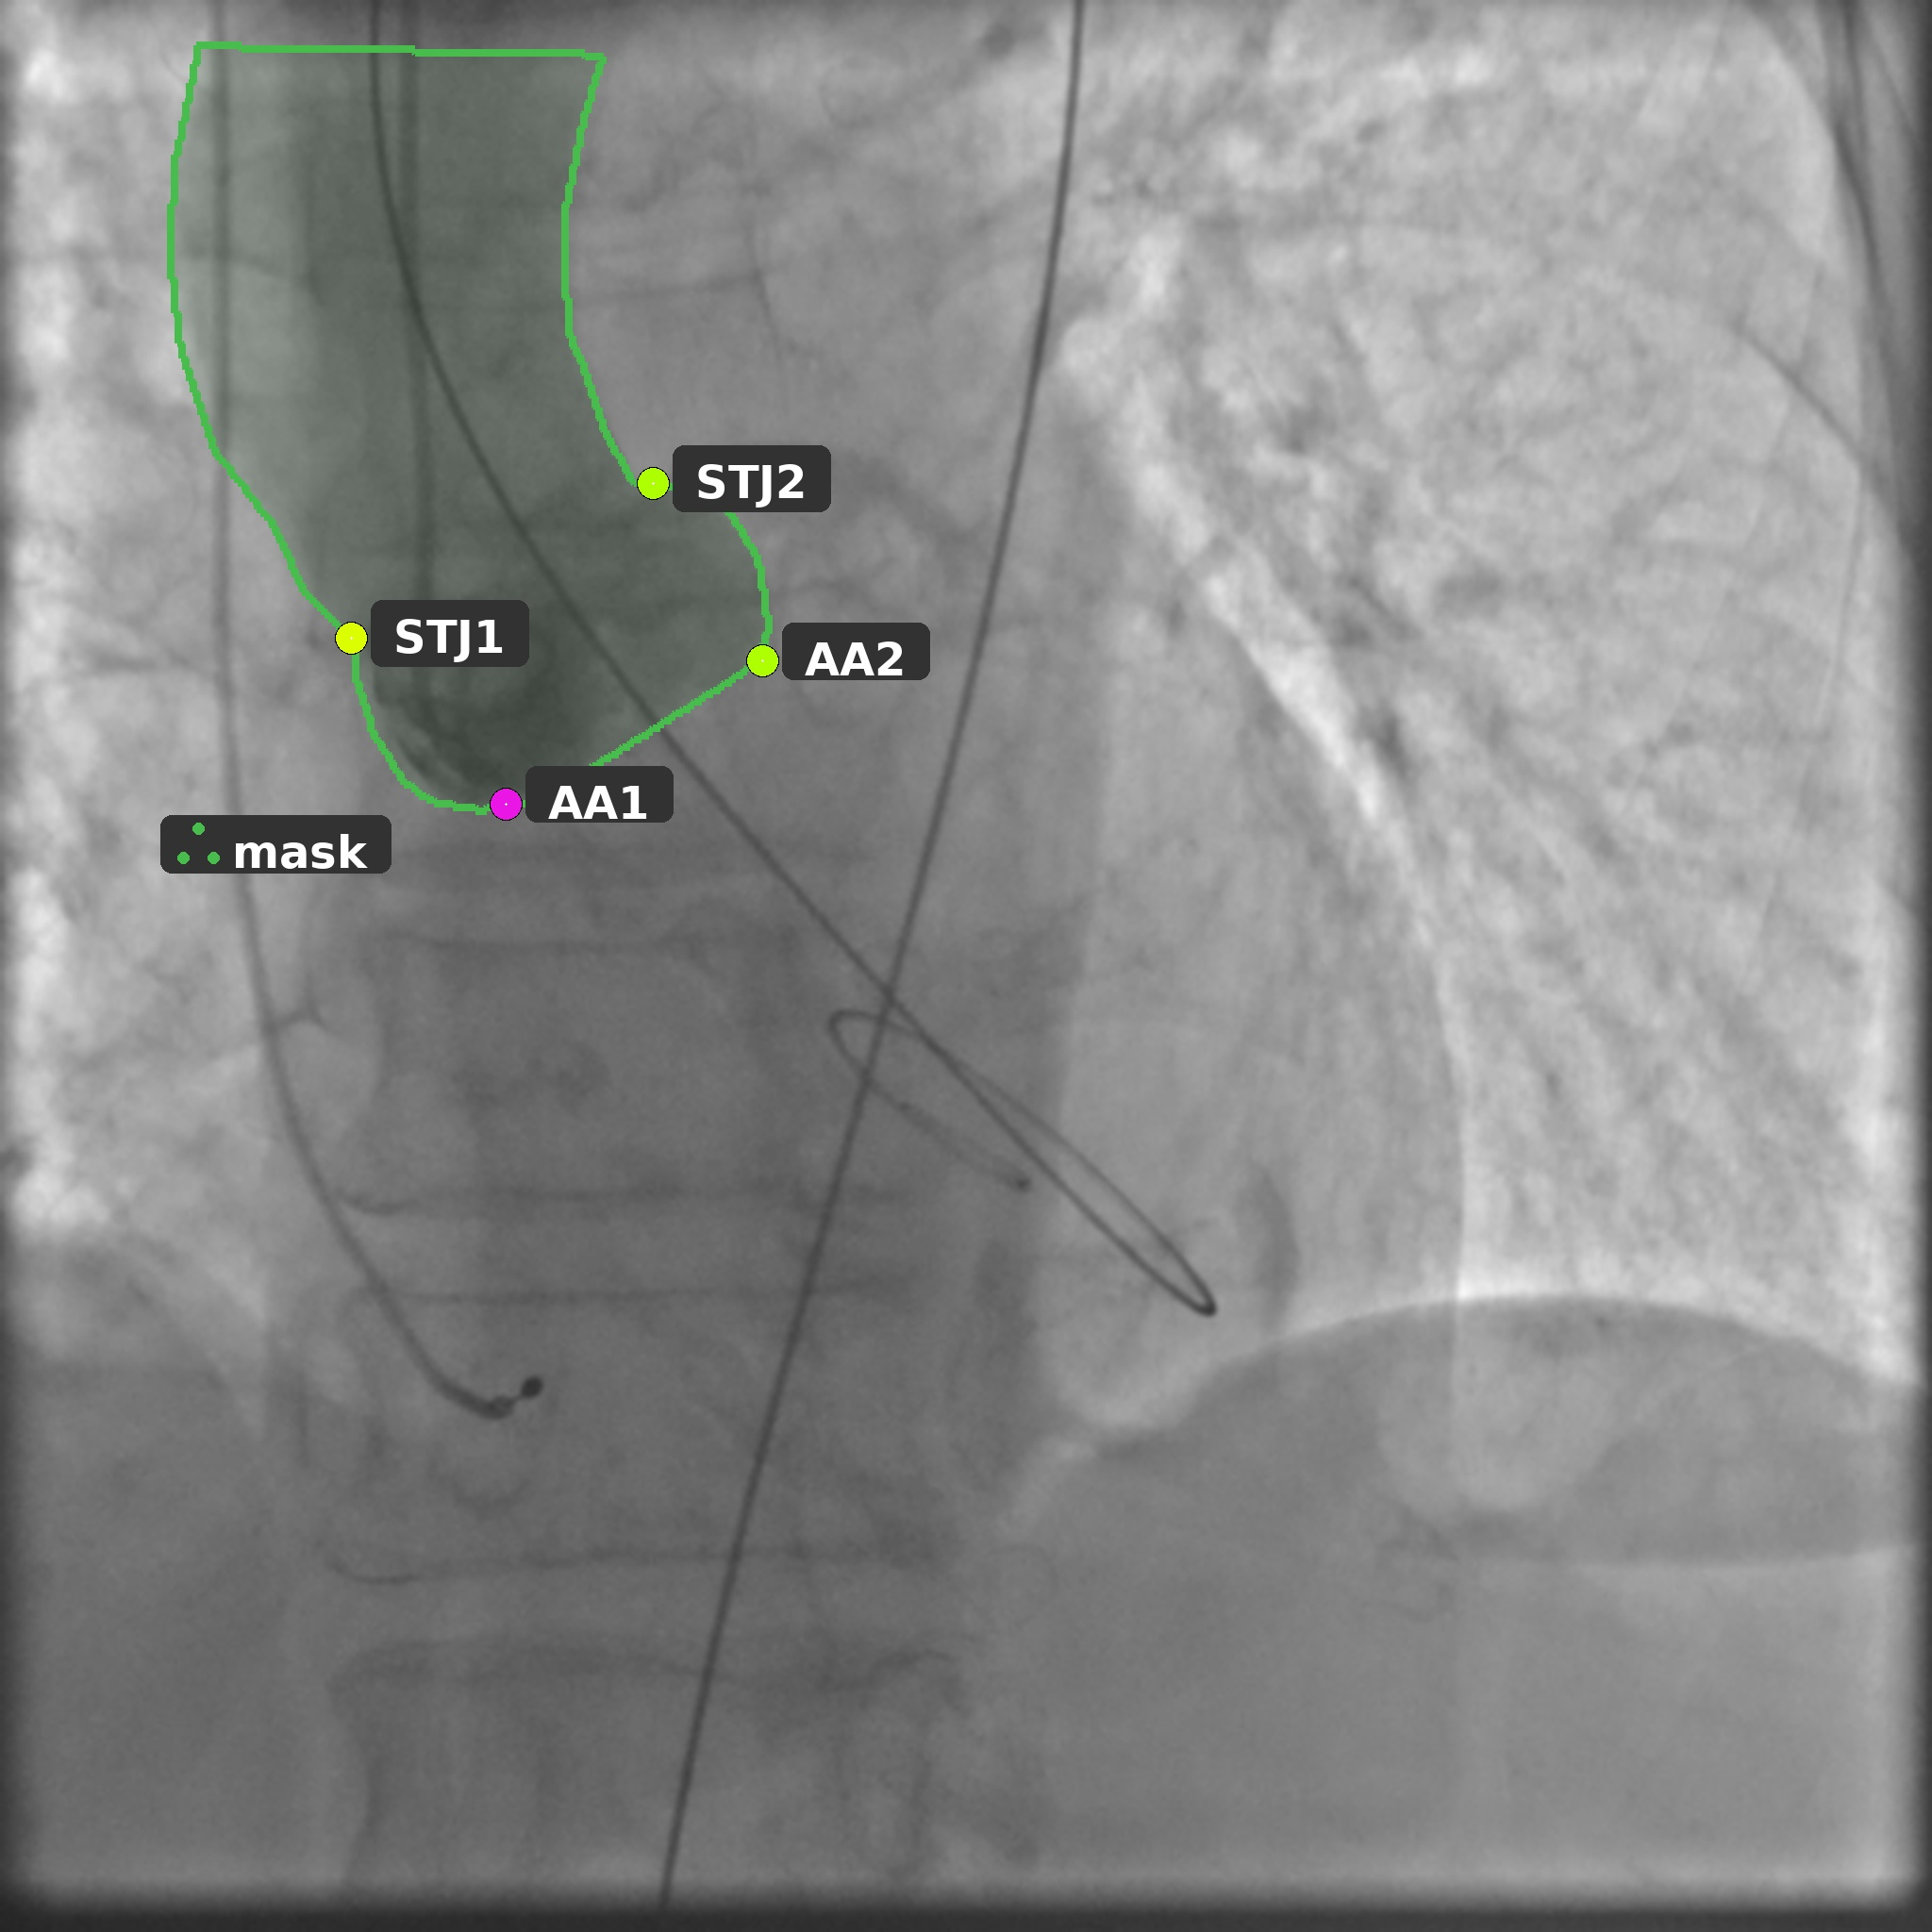
\includegraphics[width=\linewidth]{figures/Figure_1d.jpeg}
\end{minipage}
\caption{Representative fluoroscopic images (a, c) and corresponding expert annotations (b, d) illustrating the aortic root mask and four anatomical landmarks (AA1, AA2, STJ1, STJ2).}
\label{fig:S1}
\end{figure}

\begin{figure}[htbp]
\centering
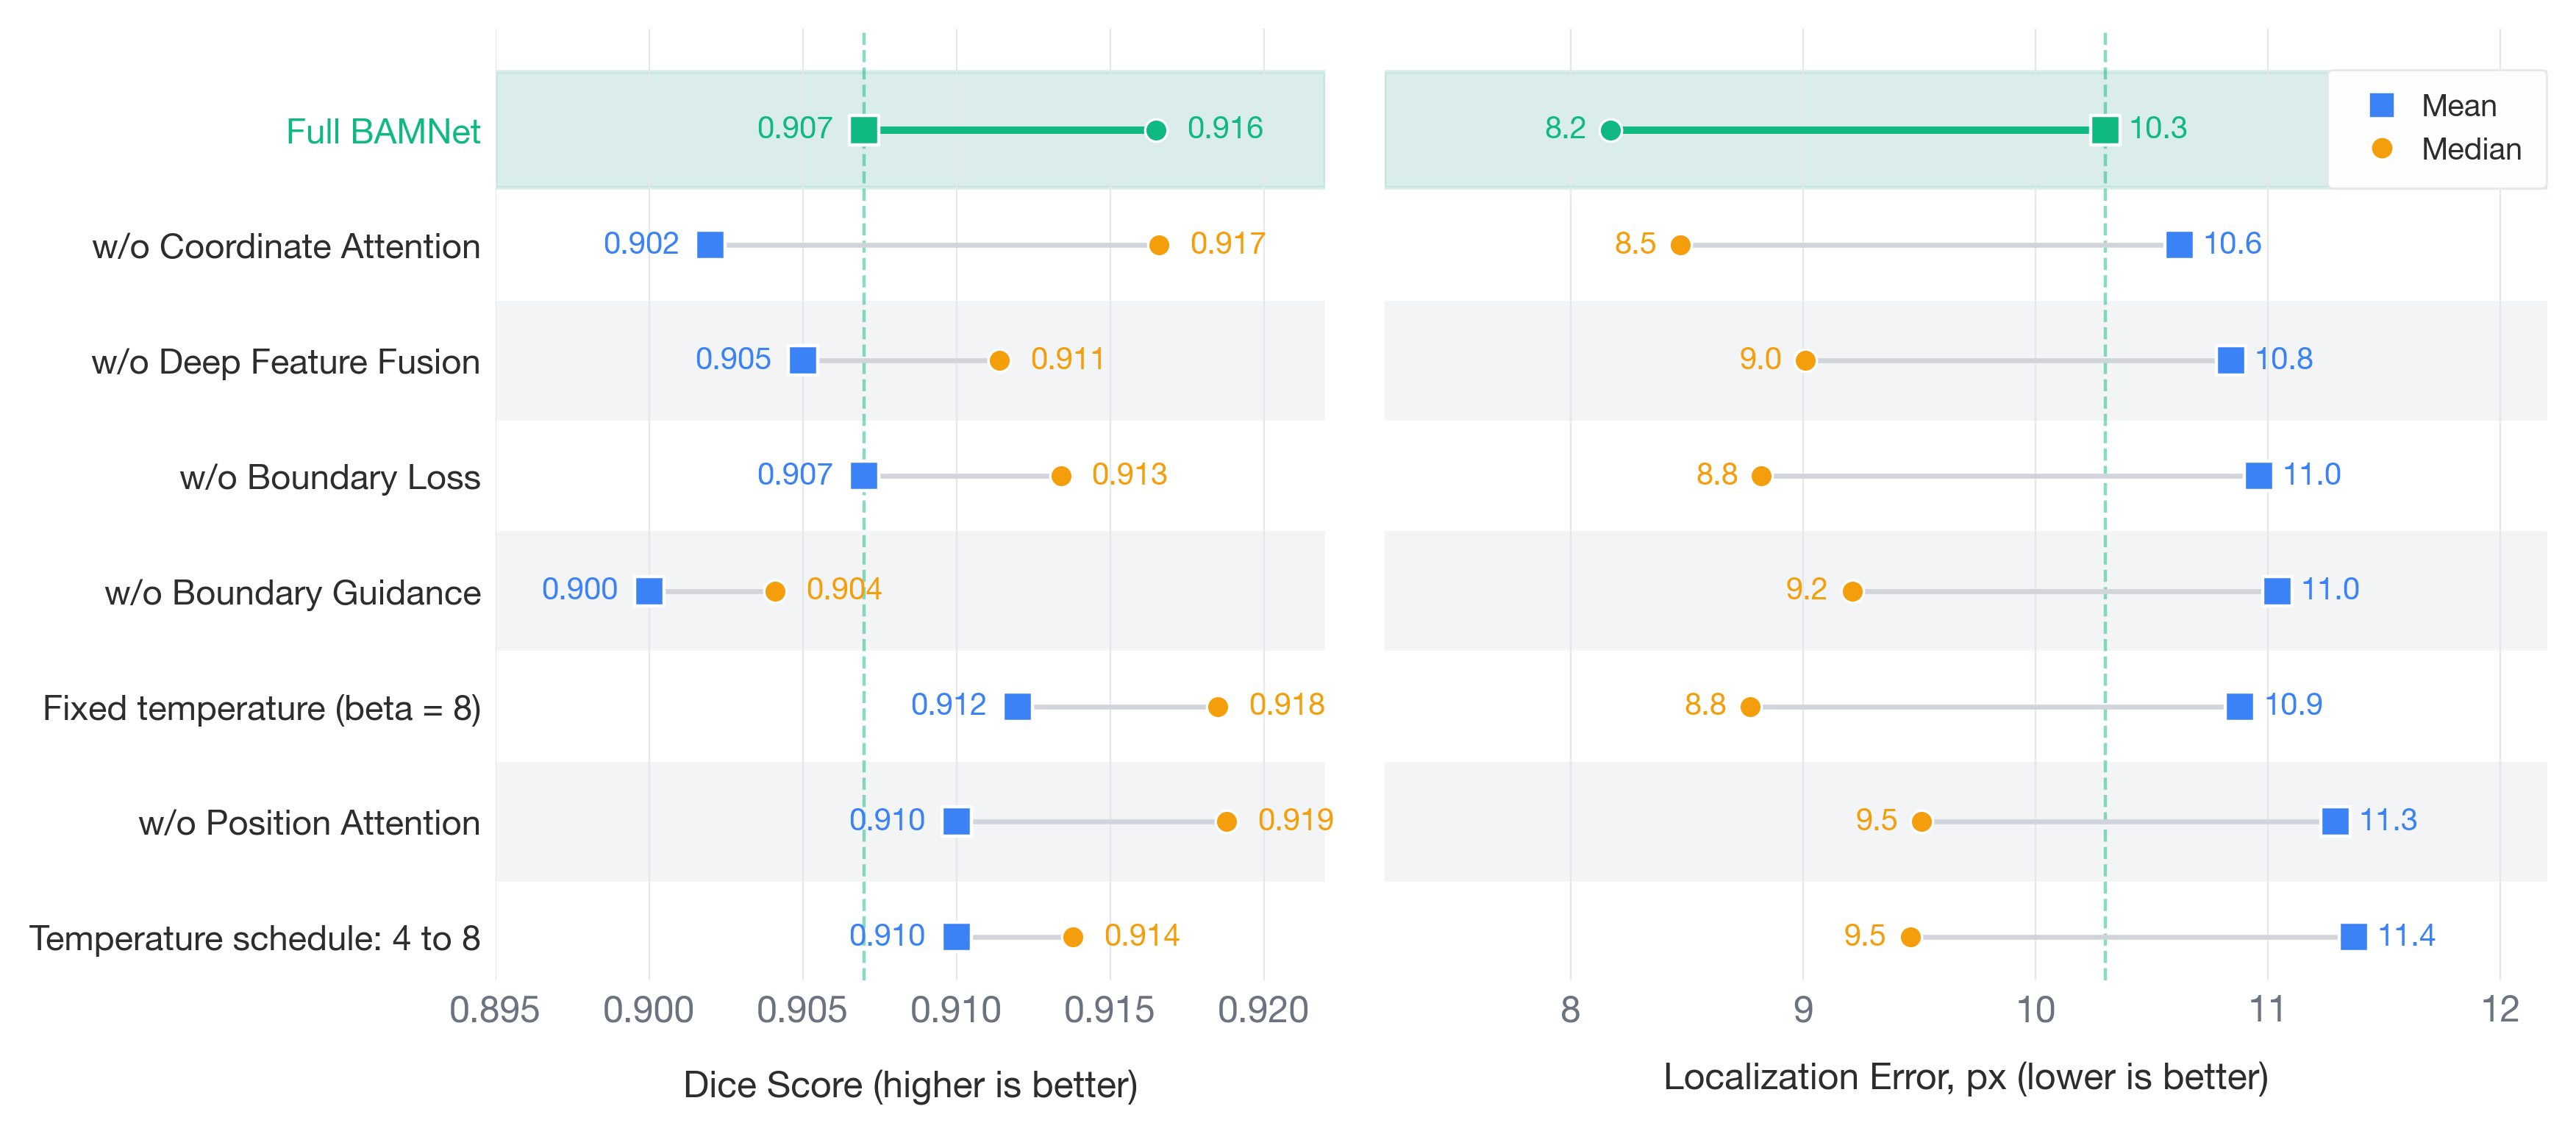
\includegraphics[width=\textwidth]{figures/Figure_4.png}
\caption{Summary of the BAMNet ablation study across the main architectural variants. The figure highlights how global spatial attention, coordinate-aware modulation, feature fusion, boundary-related supervision, and the soft-argmax configuration affect the balance between segmentation quality and landmark localization accuracy.}
\label{fig:S2}
\end{figure}

\section{Supplementary Tables}

\begin{table}[htbp]
\caption{Landmark-wise localization accuracy aggregated over five folds. Pixel errors are reported in the $640 \times 640$ model error space; millimeter errors were computed using image-specific DICOM-derived spacing rescaled to the same space.}
\label{tab:S1}
\centering
\resizebox{\textwidth}{!}{%
\begin{tabular}{lccccc}
\toprule
Landmark & Mean err. (px) & Median err. (px) & Std. err. (px) & Mean err. (mm) & Median err. (mm) \\
\midrule
AA1 & $7.96 \pm 0.73$ & $5.92 \pm 0.40$ & $7.66 \pm 1.61$ & $2.11 \pm 0.16$ & $1.57 \pm 0.09$ \\
AA2 & $11.89 \pm 0.62$ & $9.95 \pm 1.37$ & $8.60 \pm 1.00$ & $3.15 \pm 0.16$ & $2.64 \pm 0.36$ \\
STJ1 & $10.20 \pm 0.87$ & $7.66 \pm 0.14$ & $8.86 \pm 2.20$ & $2.70 \pm 0.18$ & $2.03 \pm 0.06$ \\
STJ2 & $10.02 \pm 1.46$ & $7.73 \pm 0.93$ & $8.28 \pm 2.01$ & $2.67 \pm 0.46$ & $2.06 \pm 0.31$ \\
\bottomrule
\end{tabular}}
\end{table}

\begin{table}[htbp]
\caption{Per-fold landmark localization errors for BAMNet after pixel-to-millimeter conversion. Values are reported as mean / median error in millimeters for each landmark.}
\label{tab:S2}
\centering
\resizebox{\textwidth}{!}{%
\begin{tabular}{lcccc}
\toprule
Fold & AA1 mean / median (mm) & AA2 mean / median (mm) & STJ1 mean / median (mm) & STJ2 mean / median (mm) \\
\midrule
1 & 2.13 / 1.53 & 3.39 / 3.19 & 2.50 / 1.96 & 2.79 / 2.01 \\
2 & 1.90 / 1.50 & 3.19 / 2.56 & 2.56 / 2.11 & 3.42 / 2.60 \\
3 & 2.33 / 1.64 & 3.16 / 2.74 & 2.71 / 2.04 & 2.33 / 1.91 \\
4 & 2.16 / 1.68 & 3.11 / 2.48 & 2.94 / 2.04 & 2.33 / 1.82 \\
5 & 2.02 / 1.48 & 2.93 / 2.22 & 2.80 / 2.01 & 2.46 / 1.94 \\
\bottomrule
\end{tabular}}
\end{table}

\begin{table}[htbp]
\caption{Numerical results of the BAMNet ablation study across the main architectural variants. Evaluated on fold-1 fixed hold-out test set.}
\label{tab:S3}
\centering
\resizebox{\textwidth}{!}{%
\begin{tabular}{lccccccc}
\toprule
Variant & Dice & IoU & Surface Dice@4 mm & Mean err. (px) & Median err. (px) & PCK@10 (\%) & FPS \\
\midrule
Full & 0.91 & 0.83 & 0.84 & \textbf{10.30} & \textbf{8.17} & \textbf{59.88} & 63 \\
No Pos Attn & 0.91 & 0.84 & 0.83 & 11.29 & 9.51 & 52.98 & \textbf{69} \\
No Coord Attn & 0.90 & 0.83 & 0.83 & 10.62 & 8.47 & 57.41 & 67 \\
No Fusion & 0.91 & 0.83 & 0.83 & 10.84 & 9.01 & 55.76 & 65 \\
No Bnd Guid & 0.90 & 0.82 & 0.82 & 11.04 & 9.21 & 53.70 & 66 \\
No Bnd Loss & 0.91 & 0.84 & 0.83 & 10.96 & 8.82 & 54.73 & 64 \\
Fixed 8 & \textbf{0.91} & \textbf{0.84} & \textbf{0.84} & 10.88 & 8.77 & 56.69 & 66 \\
Sched 4$\rightarrow$8 & 0.91 & 0.84 & 0.83 & 11.37 & 9.46 & 53.29 & 66 \\
\bottomrule
\end{tabular}}
\end{table}

\begin{table}[htbp]
\caption{Patient-level paired Wilcoxon signed-rank tests for the primary endpoints with Holm--Bonferroni correction. The segmentation endpoint was Dice, whereas the landmark endpoint was mean landmark error in millimeters. Metrics were first averaged within each patient.}
\label{tab:S4}
\centering
\scriptsize
\resizebox{\textwidth}{!}{%
\begin{tabular}{llllcc}
\toprule
\multicolumn{1}{c}{\raisebox{0.\baselineskip}{Endpoint}} & \multicolumn{1}{c}{\raisebox{0.5\baselineskip}{Model 1}} & \multicolumn{1}{c}{\raisebox{0.5\baselineskip}{Model 2}} & \multicolumn{1}{c}{\raisebox{0.5\baselineskip}{Raw $p$}} & \multicolumn{1}{c}{\raisebox{0.5\baselineskip}{Holm $p$}} & \shortstack{Significant\\($\alpha=0.05$)} \\
\midrule
Segmentation & BAMNet & MA-Net & $7.81 \times 10^{-2}$ & $1.56 \times 10^{-1}$ & No \\
Segmentation & BAMNet & Swin-Unet & $7.81 \times 10^{-3}$ & $3.13 \times 10^{-2}$ & Yes \\
Segmentation & BAMNet & YOLO-seg-26l & $7.81 \times 10^{-3}$ & $3.13 \times 10^{-2}$ & Yes \\
Segmentation & BAMNet & YOLO-seg-26m & $3.13 \times 10^{-1}$ & $3.13 \times 10^{-1}$ & No \\
\midrule
Landmark & BAMNet & RT-DETR & $2.34 \times 10^{-2}$ & $4.69 \times 10^{-2}$ & Yes \\
Landmark & BAMNet & YOLO-detect-26l & $7.81 \times 10^{-3}$ & $3.91 \times 10^{-2}$ & Yes \\
Landmark & BAMNet & YOLO-detect-26m & $7.81 \times 10^{-3}$ & $3.91 \times 10^{-2}$ & Yes \\
Landmark & BAMNet & YOLO-keypoints-26l & $7.81 \times 10^{-3}$ & $3.91 \times 10^{-2}$ & Yes \\
Landmark & BAMNet & YOLO-keypoints-26m & $2.34 \times 10^{-2}$ & $4.69 \times 10^{-2}$ & Yes \\
\bottomrule
\end{tabular}}
\end{table}

\end{document}
